\section{Results}

In this section we discuss the implications of our optimization framework and model of human behavior for the optimization of
\begin{enumerate*}[itemjoin*={{, and }}, itemjoin={{, }}]
    \item the number of samples captured
    \item the total energy consumption
\end{enumerate*}
per step in a \gls{WCA} task.
To this end, we introduce here three reference schemes to which we will compare our approach.

Our first reference scheme corresponds to the heuristic, state-of-the-art adaptive sampling approach introduced in~\cite{wang2019towards}.
In this work, the authors introduce an adaptive sampling scheme for \gls{WCA} intended to reduce the number of samples processed per step while still meeting application responsiveness bounds.
At every sampling instant \( t \), the scheme adapts the sampling rate of the system according to the estimated likelihood of the user having finished the step.
They express this adaptive sampling rate \( R(t) \) as
\begin{equation}
    R(t) = R_\text{min} + \varphi\left( R_\text{max} - R_\text{min} \right) * CDF(t)
\end{equation}
\( R_\text{max} \) and \( R_\text{min} \) correspond to the maximum and minimum sampling rates of the system, respectively.
\( R_\text{max} \) can directly be assumed to correspond to \( 1 / \text{\gls{RTT}}_\mu \), where \( \text{\gls{RTT}}_\mu \) corresponds to the mean \gls{RTT} of the system.
\( R_\text{min} \) needs to either be calculated according to the latency bounds of the system or specified manually.
\( \varphi \) corresponds to a scaling factor and \( t \) to the time of the current sampling instant with respect to the start of the step.
\( CDF \) corresponds to the \gls{CDF} of a Gaussian distribution describing the execution times for the current step.

We also implement two reference sampling schemes representing best- and worst-case extremes.
The first of these corresponds to the offline optimum which uses an embedded \emph{oracle} to perfectly predict the execution time of each step.
Such an ideal scheme is thus able to always sample exactly once per step, with a constant wait time of zero.
The third and final reference scheme corresponds to one which \emph{greedily} samples as much as possible.
This represents a completely unoptimized design with no considerations for resource-consumption trade-offs; it simply attempts to maximize the number of captured samples per step.
This is an interesting approach to include as it corresponds to the sampling strategy used in most existing \gls{WCA} prototypes.

In the following, we will show the effects of our optimization approach combined with our timing models compared to the reference schemes.
We implement all sampling schemes in Python and run a number of simulations with them.
Our approach is based on \cref{eq:tnRayleigh,eq:tnRayleigh:energy,eq:tnRayleigh:samples} to determine quasi-optimum sampling instants at each step.
It includes an embedded timing model outputting an empirical distribution to provide updated estimates of the execution time \( \mu \) and \( \sigma \), allowing it to adapt to the state of the system.

\subsection{Optimizing for number of samples}\label{ssec:optimization:samples}
\todo[inline]{TODO}

\begin{table}
    \centering
    \caption{Experimental parameters}\label{tab:params}
    \begin{tabular}{lrl}
        \toprule
        Parameter & Value & Clarification \\
        \midrule
        \# of steps & \num{100} & \\
        Repetitions & \num{100} & \\
        \glspl{RTT} & \( \left\{ 0.3, 0.6,\ldots,4.2 \right\} \) & \\
        \( \tau_\text{p} \) & \SI{250}{\milli\second} & Processing delay \\
        \( \tau_\text{c} \) & \( \text{\gls{RTT}} - \tau_\text{p} \) & Communication delay \\
        \( w_0 \) & \SI{1.0}{\second} & \\
        \( R_\text{min} \) & \SI{0.5}{\hertz} & Derived as \( R_\text{min} = {(2 w_0)}^{-1} \) \\
        \( \varphi \) & \num{1.5} & Scaling factor, \textcite{wang2019towards}\\
        \( P_0 \) & \SI{15}{\milli\watt} & Idle power \\
        \( P_\text{c} \) & \SI{45}{\milli\watt} & Communication power \\
        \( \alpha_\text{samples} \) & \( 1.9 \sigma^{-1} \) & For sample-count optimization. \\
        \( \beta_\text{samples} \) & \num{1.0} & For sample-count optimization. \\
        \( \alpha_\text{energy} \) & \( \tau_\text{c}(P_\text{c} - P_0) \) & For energy optimization. \\
        \( \beta_\text{energy} \) & \( P_0 \) & For energy optimization. \\
        \bottomrule
    \end{tabular}
\end{table}

We proceed to set up an experiment where these sampling approaches are deployed on identical, simulated, tasks with varying constant \glspl{RTT}.
Experimental parameters are summarized in \cref{tab:params}.
We set the \( w_0 \) and \( \beta \) factors of our sample-count-optimized scheme to \SI{1.0}{\second} and \num{1.0}, respectively, for mathematical simplicity, and derive \( \alpha = 1.9 \sigma^{-1} \).
Next, we derive \( R_\text{min} \) for \textcite{wang2019towards}'s scheme from \( w_0 \).
As discussed in \cref{sec:background}, we assume that wait times are uniformly distributed between \SI{0}{\second} and sampling interval of each step.
A maximum expected wait time \( w_0 = 1.0\,\si{\second} \) thus translates into a maximum expected sampling interval of \SI{2.0}{\second}, yielding a minimum sampling rate \( R_\text{min} = {2.0\,\si{\second}}^{-1} = 0.5\,\si{\hertz} \).
It should also be noted that in both aperiodic schemes, our sampling-count-optimized approach and the \gls{CDF}-based approach, there exists the possibility for sampling instants to be \emph{missed} due to the actual \gls{RTT} of the system being higher than the parameterization of the schemes.
In these cases, both schemes will degrade into greedy sampling.

The execution times for each step are generated by a timing model without any distribution fitting on the data.
For each combination of sampling scheme configuration, \gls{RTT}, and execution time model neuroticism (low or high), we run \num{100} repetitions of the task for good statistical significance.
Note that the embedded timing model in our sampling-count-optimized aperiodic sampling scheme is always parameterized with a neuroticism matching the neuroticism of the external execution time model.

\begin{figure*}
    \centering
    \begin{subfigure}[t]{\textwidth}
        \centering
        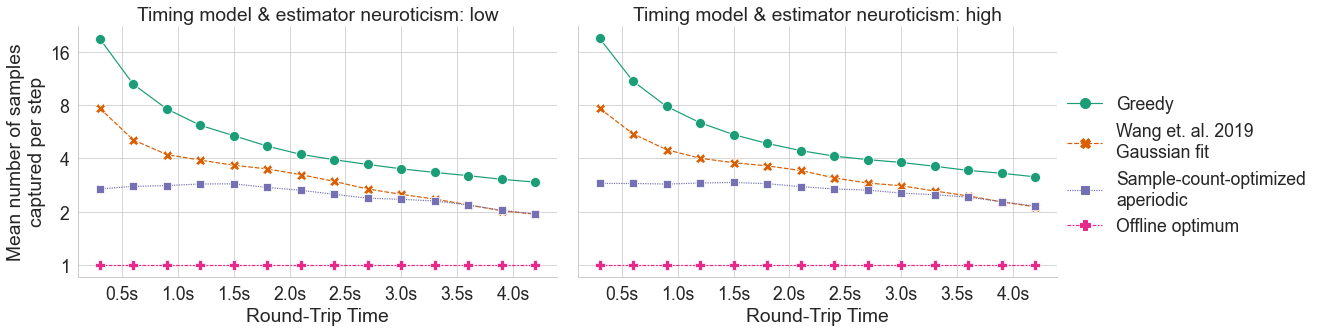
\includegraphics[width=\textwidth]{figs/new_model/sampling_optimization.png}
        \caption{%
            Round-trip time versus mean number of captured samples per step, averaged over all \num{100} repetitions of the experiment.
            Note the logarithmic scale on the vertical axis.
            Error bars indicate \SI{95}{\percent} \glspl{CI}.
        }
    \end{subfigure}\\
    \medskip
    \begin{subfigure}[t]{\textwidth}
        \centering
        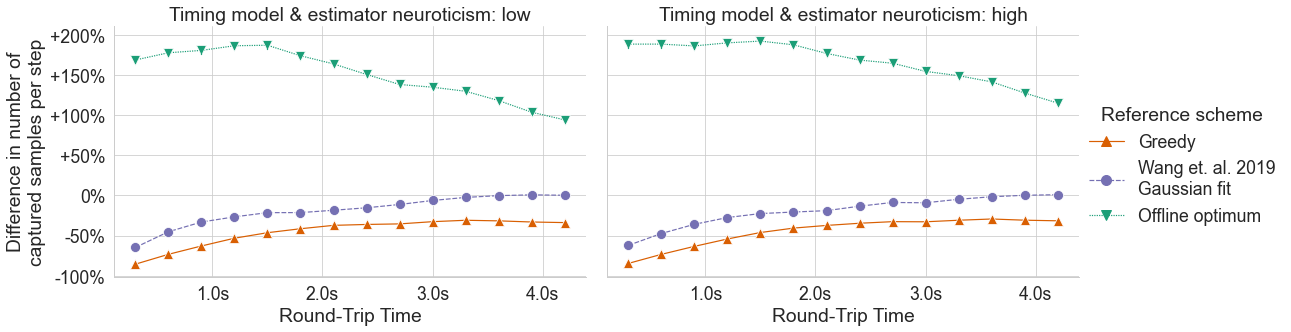
\includegraphics[width=\textwidth]{figs/new_model/sampling_optimization_diff.png}
        \caption{%
            Percentage difference in mean number of captured samples per step by the sample-count-optimized approach with respect to the three reference schemes.
            In other words, curves represent the relative performance of the sample-count-optimized scheme when using the corresponding reference scheme as baseline.
            Error bars indicate \SI{95}{\percent} \glspl{CI}, calculated using a two-sided t-test.
        }
    \end{subfigure}
    \caption{%
        Summary of results for experiment comparing the sample-count-optimized aperiodic sampling scheme to the reference schemes and \textcite{wang2019towards}'s \gls{CDF}-based approach.
    }\label{fig:optimization:samples}
\end{figure*}

The results of this investigation are presented in \cref{fig:optimization:samples}, and clearly show the advantages of using the sample-count-optimized scheme over the current state-of-the-art.
The performance of \textcite{wang2019towards}'s approach appears to degrade with lower \glspl{RTT}, exponentially oversampling as latency tends to zero and the maximum sampling rate of the system tends to infinity.
On the other hand our sampling scheme consistently matches or beats the state-of-the-art while maintaining a relatively constant behavior with respect to \glspl{RTT}.
As mentioned above, the future feasibility and mass adoption of \gls{WCA} depends on these applications not hogging the available resources.
Our work advances this goal by being consistently more efficient than existing alternatives at minimizing the number of samples per step, and thus reducing network and processing load.

It should be noted that although both schemes seem to tend towards two samples per step as \glspl{RTT} increase, this is simply an artifact of our experimental setup.
As \glspl{RTT} increase above the expected wait time, the probability of the sum of the first sampling interval and the \gls{RTT} being larger than the execution time of the step tends towards \num{1.0}.
This leads to these sampling schemes consistently sampling only twice each step: a first sample which is taken before the execution time of the step, and a second one \gls{RTT} seconds later, after the execution time has been reached.

\subsection{Optimizing for energy consumption}\label{ssec:optimization:energy}

We proceed to repeat the experiment detailed in \cref{ssec:optimization:samples}, replacing the sample-count-optimized sampling scheme with a new implementation instead minimizing energy, using \cref{eq:optimization:energy} for the calculation of \( \alpha \) and \( \beta \).
Once again, we embed a timing model into the sampling scheme to provide updated estimates of the mean execution time \( \mu \) at each step.
We refer to this scheme as the \emph{energy-optimized aperiodic} sampling scheme.
For the power constants, we reuse the values estimated by the authors in~\cite{moothedath2022energy1}, \( P_\text{c} = 45\,\si{\milli\watt} \) and \( P_\text{0} = 15\,\si{\milli\watt} \).
On the other hand, for the timing variables we define a constant processing delay \( \tau_\text{p} = 250\,\si{\milli\second} \) across all configurations and repetitions of the experiments; given then a constant \gls{RTT} for the task, we set \( \tau_\text{c} = \text{\gls{RTT}} - \tau_\text{p} \).

\begin{figure*}
    \centering
    \begin{subfigure}[t]{\textwidth}
        \centering
        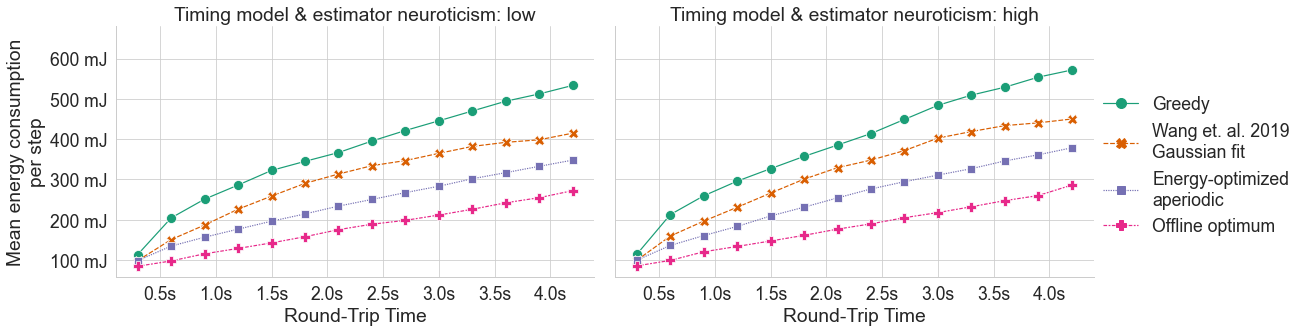
\includegraphics[width=\textwidth]{figs/new_model/energy_optimization.png}
        \caption{%
            Round-trip time versus mean per step energy consumption, averaged over all \num{100} repetitions of the experiment.
            Error bars indicate \SI{95}{\percent} \glspl{CI}.
        }
    \end{subfigure}\\
    \medskip
    \begin{subfigure}[t]{\textwidth}
        \centering
        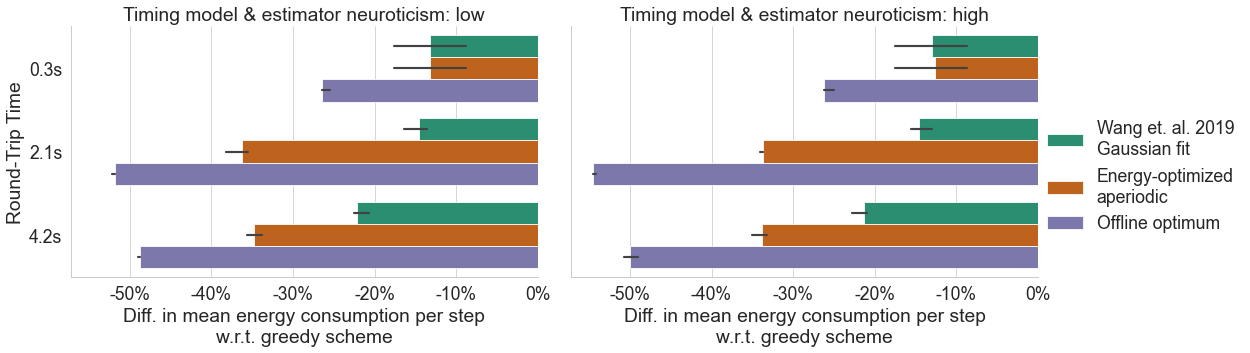
\includegraphics[width=\textwidth]{figs/new_model/energy_optimization_diff.png}
        \caption{%
            Percentage difference in mean per step energy consumption by the energy-optimized sampling scheme with respect to the three reference schemes.
            Error bars indicate \SI{95}{\percent} \glspl{CI}, calculated using a two-sided t-test.
        }
    \end{subfigure}
    \caption{%
        Summary of results for experiment comparing the energy-optimized aperiodic sampling scheme to the reference schemes and \textcite{wang2019towards}'s \gls{CDF}-based approach.
    }\label{fig:optimization:energy}
\end{figure*}

Again, we include the reference greedy and offline optimum schemes, as well as \textcite{wang2019towards}'s approach, and repeat the experiment \num{100} times for each combination of sampling scheme, neuroticism, and \gls{RTT}.

The results of these experiments are presented in \cref{fig:optimization:energy}, and they clearly illustrate the advantages of the integration of our timing models with an adaptive, energy-optimized sampling scheme when compared to unoptimized and state-of-the-art sampling schemes.
Our approach is consistently consumes \SI{20}{\percent} less energy than \textcite{wang2019towards}'s state-of-the-art, and is up to \SI{40}{\percent} more energy efficient than the greedy scheme.
Furthermore, once again the behavior of our approach is more consistent and reliable than the competition, exhibiting a flat curve of energy consumption much akin to that of the offline optimum in behavior.
